\documentclass{article}

\usepackage{amsmath, amsthm, amssymb, amsfonts}
\usepackage{thmtools}
\usepackage{graphicx}
\usepackage{setspace}
\usepackage{geometry}
\usepackage{float}
\usepackage{hyperref}
\usepackage[utf8]{inputenc}
\usepackage[spanish]{babel}
\usepackage{framed}
\usepackage[dvipsnames,table,xcdraw]{xcolor}
\usepackage{tcolorbox}
\usepackage{wrapfig}
\usepackage{multirow}
\usepackage{pifont}

\colorlet{LightGray}{White!90!Periwinkle}
\colorlet{LightOrange}{Orange!15}
\colorlet{LightGreen}{Green!15}

\newcommand{\HRule}[1]{\rule{\linewidth}{#1}}

\DeclareMathAlphabet\mathbfcal{OMS}{cmsy}{b}{n}

\declaretheoremstyle[name=Theorem,]{thmsty}
\declaretheorem[style=thmsty,numberwithin=section]{theorem}
\tcolorboxenvironment{theorem}{colback=LightGray}

\declaretheoremstyle[name=Proposition,]{prosty}
\declaretheorem[style=prosty,numberlike=theorem]{proposition}
\tcolorboxenvironment{proposition}{colback=LightOrange}

\declaretheoremstyle[name=Principle,]{prcpsty}
\declaretheorem[style=prcpsty,numberlike=theorem]{principle}
\tcolorboxenvironment{principle}{colback=LightGreen}

\setstretch{1.2}
\geometry{
    textheight=9in,
    textwidth=5.5in,
    top=1in,
    headheight=12pt,
    headsep=25pt,
    footskip=30pt
}

% ------------------------------------------------------------------------------

\begin{document}

% ------------------------------------------------------------------------------
% Cover Page and ToC
% ------------------------------------------------------------------------------

\title{ \normalsize \textsc{}
\\ [2.0cm]
\HRule{1.5pt} \\
\LARGE \textbf{\uppercase{CheatSheet ANDA}
\HRule{2.0pt} \\ [0.6cm] \LARGE{Formulas y resultados para la asignatura de Analisis de Datos} \vspace*{10\baselineskip}}
}
\date{}
\author{\textbf{Autor} \\
    Victor Elvira Fernández, Tomás Ruiz Rojo, Juan Horrillo Crespo \\
    Universidad de Valladolid \\
    \date{\today}
}

\maketitle
\newpage

\begin{center}
    \Huge \textbf{AVISO}
\end{center}

Estos apuntes fueron creados de forma voluntaria por un grupo de estudiantes, invirtiendo tiempo, dedicación y esfuerzo para ofrecer información útil a la comunidad. Apreciamos cualquier apoyo que se nos quiera brindar, ya que nos ayuda a continuar con futuros proyectos de este tipo. \\

Si deseas colaborar en esta clase de proyectos puedes contactarnos y unirte o invitarnos a unas ricas patatas 5 salsas por el siguiente enlace:

\vfil

\begin{center}
    \href{https://www.buymeacoffee.com/ApuntesINdat}{\LARGE \textbf{Buy Me a Patatas 5 Salsas}}
    \href{https://www.buymeacoffee.com/ApuntesINdat}{https://www.buymeacoffee.com/ApuntesINdat}
\end{center}

\begin{itemize}
    \item \href{mailto:juan.horrillo22@estudiantes.uva.es}{Mail Juan Horrillo}
    \item \href{mailto:victor.elvira22@estudiantes.uva.es}{Mail Victor Elvira}
    \item \href{mailto:tomas.rojo22@estudiantes.uva.es}{Mail Tomás Rojo}
\end{itemize}

\vfil

Si has colaborado de cualquier forma te agradecemos enormemente.
\newpage

\tableofcontents
\newpage
\null
\newpage

% ------------------------------------------------------------------------------

\section{Análisis por Componentes Principales}

\begin{itemize}
    \item Matriz de datos:
          \[X_{n \times k} = \begin{bmatrix}x_{11} & x_{12} & \cdots & x_{1k} \\ x_{21} & x_{22} & \cdots & x_{2k} \\ \vdots & \vdots & \ddots & \vdots \\ x_{n1} & x_{n2} & \cdots & x_{nk}\end{bmatrix}\]
    \item Individuo: Punto de $\mathbb{R}^k$
    \item Variable: Punto de $\mathbb{R}^n$
    \item Inercia Total: Suma de la distancia cuadrada de las observaciones al centro de gravedad G (lo situamos en 0)
          \[I_t = \sum_{i=1}^{n}d^2(x_i, G) = \sum_{i=1}^{n}(x_i-G)'(x_i-G) = \sum_{i=1}^{n}\left\lVert x_i \right\rVert^2 = tr(XX') = tr(X'X)\]
    \item Inercia explicada por $u$: Inercia explicada por el resumen unidimensional de los datos proyectados sobre $u$.
    \item $I_t = \sum_{i=1}^{k}I_{u_i}$
    \item El mayor autovector $u_1$ de $X'X$ maximiza la inercia recogida de entre cualquier otro vector.
    \item El siguiente mayor autovector $u_2$ de $X'X$ es el que recoge más inercia por detras de $u_2$.
    \item Sean $u_1, \dots, u_k$ los autovectores de $X'X$ entonces se verifica que $I_{u_1} \geq \dots \geq I_{u_k}$
    \item Descomposición en valores singulares: Sea $M$ matriz $k\times k$ simétrica definida no negativa. Entonces existe una matriz $U$ ortonormal tal que
          \[U'MU = \Delta\]
          con $\Delta = diag(\lambda_1, \dots, \lambda_k)$ y $\lambda_1 \geq \dots \geq \lambda_k \geq 0$.
    \item En nuestro caso $M = X'X$, por tanto $U$ esta formada por los autovectores que estamos buscando y $\lambda_i$ son los autovalores correspondientes.
    \item Como $tr(M) = tr(\Delta)$ se deduce que $I_t = tr(X'X) = tr(\Delta) = \sum_{i=1}^{k}\lambda_i$. O lo que es lo mismo, $I_{u_i} = \lambda_i$.
    \item Componente principal: Se define como componente principal de la siguiente forma \[F_\alpha = u_{1\alpha}X_1 + \dots + u_{k\alpha}X_k\]
          \newpage
    \item La proyección de un individuo $i$ sobre el eje $\alpha$ sería $F_{i\alpha} = x_i'u_\alpha$.
    \item Analisis Normado: Permite realizar analisis de forma que lo que se descubra no sea la diferencia entre las varianzas de las variables. Entre otras cosas, es util para comparar mediciones de distintas unidades.
    \item Sea $X^*$ una matriz de datos estandarizada, entonces la matriz $\frac{1}{n-1}(X^*)'X^*$ contiene no las covarianzas sino las correlaciones muestrales.
    \item Inercia acumulada: $I.a._s = \sum_{i=1}^{s}I_i$
    \item Porcentaje de inercia acumulada: $100\frac{\sum_{i=1}^{s}I_i}{\sum_{i=1}^{k}I_i} = 100\frac{I.c_s}{I_t}$
    \item Algunos criterios de retención de componentes:
          \begin{itemize}
              \item Considerar el porcentaje de inercia acumulado y decidir retener un numero de componentes s que haga que la inercia explicada supere un determinado porcentaje.
              \item Extraer aquellas componentes cuya inercia explicada supere el promedio de los autovalores (en el caso normado habitual esto es equivalente a extraer las componentes con autovalores mayores que 1).
              \item Construir el denominado "scree plot" en el que se representa en el eje de ordenadas el número del autovalor y en el de abcisas el autovalor en si y buscar el codo del gráfico.
          \end{itemize}
    \item Contribuciones absolutas (a la inercia explicada por cada eje): Se definen como $c.a.(i,\alpha)=\frac{(x_i'u_\alpha)^2}{(n-1)\lambda_\alpha}$. Nos dice lo que ha contribuido el individuo $i$ a la definición del eje $\alpha$.
    \item $\sum_{i=1}^{n}c.a.(i,\alpha)=1$ por lo que si un punto tiene contribuciones mucho más altas que el resto podemos dudar de la estabilidad del eje, ya que puede estar excesivamente condicionado por ese punto.
    \item Contribuciones relativas (cosenos cuadrados): Se definen como $c.r.(i,\alpha)=\cos^2(i,\alpha)=\frac{(x_i'u_\alpha)^2}{d^2(i,G)}$. Nos dicen como de cerca (o lejos) esta un punto de cada eje. Sirve para saber si un punto está mejor o peor representado en un eje o conjunto de ejes.
    \item $\sum_{\alpha=1}^{k}\cos^2(i,\alpha)=1$
    \item Análisis de la nube de variables: Análisis como el anterior pero sobre la matriz transpuesta $X'_{(k\times n)}$. Por tanto buscamos un vector $v\in\mathbb{R}^n$
    \item Como $(X'X)_{(k\times k)}$ tiene el mismo rango que $(XX')_{(n\times n)}$, $XX'$ tendrá solo $k$ autovalores mayores que 0.
    \item Sea $\lambda_i$ autovalor de $X'X$ y $\mu_i$ autovalor de $XX'$ entonces $\lambda_i = \mu_i$.
    \item Sea $v_i$ autovector de $XX'$, entonces $v_i = \frac{1}{\sqrt{\lambda_i}}Xu_i$.
    \item Sea $u_i$ autovector de $X'X$, entonces $u_i = \frac{1}{\sqrt{\lambda_i}}X'v_i$.
    \item De lo que se deduce que $\sqrt{\lambda_i}u_i = X'v_i$
    \item Si se usa la matriz $\frac{1}{n-1}X'X$ las formulas correctas serán:
          \[v_i=\frac{1}{\sqrt{(n-1)\lambda_i}}Xu_i \quad u_i=\frac{1}{\sqrt{(n-1)\lambda_i}}X'v_i\]
    \item $X=V\Delta^\frac{1}{2}U'$.
    \item $\sum_{i=1}^{k}\sqrt{\lambda_i}v_iu_i'=\sum_{i=1}^{k}Xu_iu_i'=X\sum_{i=1}^{k}u_iu_i'=XUU'=X$ por tanto podemos reconstruir la matriz original a partir de los autovalores y autovectores de $X'X$ o $XX'$.
    \item Si nos quedamos con las primeras $q$ componentes podemos reproducir los datos de forma aproximada: $\tilde{X}=\sum_{i=1}^{q}\sqrt{\lambda_i}v_iu_i'=X\tilde{U}\tilde{U}'$.
    \item La inercia recogida con $\tilde{X}$ con respecto a la original es $\frac{tr(\tilde{X}'\tilde{X})}{tr(X'X)}$.
    \item Denotamos $G_\alpha = X'v_\alpha = \sqrt{\lambda_\alpha}u_\alpha$ a la proyección de las variables sobre el eje $\alpha$.
    \item En un análisis normado $Corr(X_j,F_\alpha)=G_{j\alpha}$
    \item Contribuciones absolutas (a la inercia explicada por cada eje): Se definen como $c.a.(j,\alpha) = \frac{G^2_{j\alpha}}{\lambda_\alpha}=u^2_{j\alpha}$. Nos dice lo que ha contribuido la variable $j$ a la definición del eje $\alpha$.
    \item $\sum_{j=1}^{k}c.a.(j,\alpha)=1$
    \item Contribuciones relativas (cosenos cuadrados): Se definen como $c.r.(j,\alpha)=\cos^2(j,\alpha)=\frac{G^2_{j\alpha}}{d^2(j,G)}=\frac{G^2_{j\alpha}}{Var(j)}$. Nos informan de la calida de la representación de la variable en la dimensión correspondiente.
    \item Si el análisis es normado entonces $Var(j)=1$ con lo que $c.r.(j,\alpha)=\cos^2(j,\alpha)=G^2_{j\alpha}$ o lo que es lo mismo $c.r.(j,\alpha)=\cos^2(j,\alpha)=Corr^2(X_j,F_\alpha)$.
    \item $\sum_{\alpha=1}^{k}c.r.(j,\alpha)=1$
    \item Factor tamaño: Al no estar la nube de variables centrada podría ocurrir que todas las coordenadas de las variables de un eje tengan el mismo signo. Cuando esto ocurre en el primer eje se dice que es un factor de tamaño, pues si nos movemos por él, todas las variables crecerán y las observaciones serán más grandes, por tanto teniendo mayor "tamaño".
    \item Variables Ilustrativas Continuas: Para posicionarlas se proyectan sobre los ejes igual que cualquier otra variable \[G^+_{j\alpha}=Corr(X^+_j,F_\alpha)\] si el analisis es normado y \[G^+_{j\alpha}=Var(X^+_j)Corr(X^+_j,F_\alpha)\]. La calidad de representación sobre el eje $\alpha$ será \[\cos^2(j^+,\alpha)=Corr^2(X^+_j,F_\alpha)\]. El superíndice $+$ indica que se trata de una variable ilustrativa.
    \item La suma de los cosenos cuadrados puede ser menor que 1.
    \item No tiene sentido calcular contribuciones a los ejes pues no han participado en la determinación de los mismos.
    \item Variables Ilustrativas Nominales: Lo que se hace es calcular los individuos promedio de cada una de las clases y proyectarlos sobre el análisis como el resto de los individuos.
    \item Individuos Ilustrativos: Se proyectan como el resto de individuos. Puede calcularse la calidad de su representación pero no tendrán contribuciones a los ejes.
    \item Representaciones Simultáneas: La fila j de la matriz U contiene las proyecciones de la variable j sobre los ejes. El punto variable j puede representarse en la nube de puntos individuo. Este punto es el extremo del vector que define la dirección de crecimiento de la variable j en la nube de los individuos.
    \item Algunas consideraciones al respecto:
          \begin{enumerate}
              \item Sólo la dirección de las variables cuenta en la interpretación conjunta con los individuos.
              \item Estas proyecciones estarán dentro del círculo unidad y cuanto más cerca esté el punto de la circunferencia mejor representada estará la dirección de crecimiento en el espacion en el que se trabaja.
              \item Los individuos próximos al centro de la representación tomarán valores cercanos a la media de la variable y los que estén lejos del centro en la dirección de crecimiento tomarán valores altos en esa variable.
          \end{enumerate}
    \item Técnicas de validación de la estabilidad:
          \begin{enumerate}
              \item Perturbación aleatoria de los datos: Se genera un nuevo conjunto de datos $x_{ij}=x_{ij}+N(0,K\sigma_j)$ donde $x_{ij}$ son los datos iniciales, $\sigma_j$ la desviación típìca de $j$. $K$ mide el nivel de perturbación. Se calculan las correlaciones de los ejes de los ejes de estos datos con los ejes de los datos originales. Habrá estabilidad si cada eje tiene una correlación alta con el eje del mismo orden de los datos originales.
              \item  Bootstrap: Se generan muestras bootstrap a partir del conjunto de datos original. Se efectua el ACP para cada subconjunto. Se pueden entonces construir distribuciones bootstrap para los autovalores y para las correlaciones entre los ejes iniciales y los ejes bootstrap y valorar su estabilidad.
          \end{enumerate}
\end{itemize}


\section{Análisis de Correspondencias}

\begin{itemize}
    \item Se realiza sobre variables categóricas. Se quiere estudiar relaciones entre las variables y las categorías de las mismas.
    \item Test $\chi^2$ de independencia: \[H_0:p_{ij}=p_{i+}\times p_{+j}, \quad \forall i=1,\dots,r,j=1;\dots,c\] donde \[\chi^2 = \sum_{i=1}^{r}\sum_{j=1}^{c}\frac{(n_{ij}-\frac{n_{i+}n_{+j}}{n_{++}})^2}{\frac{n_{i+}n_{+j}}{n_{++}}}=\sum_{i=1}^{r}\sum_{j=1}^{c}\frac{(Obs_{ij}-Esp_{ij})^2}{Esp_{ij}}\thicksim \chi^2_{(r-1),(c-1)}\]
    \item Perfiles fila y columna: Son las distribuciones condicionadas por filas y columnas. \[\text{Perfiles Fila: }\begin{pmatrix}\frac{n_{i1}}{n_{i+}}, & \cdots, & \frac{n_{ic}}{n_{i+}}\end{pmatrix}, \quad \forall i=1,\dots,r\] \[\text{Perfiles Columna: }\begin{pmatrix}\frac{n_{1j}}{n_{+j}}, & \cdots, & \frac{n_{rj}}{n_{+j}}\end{pmatrix}', \quad \forall j=1,\dots,c\]
    \item Si consideramos las frecuencias relativas $f_{ij}=\frac{n_{ij}}{n_{++}}$, $f_{i+}=\frac{n_{i+}}{n_{++}}$ y $f_{+j}=\frac{n_{+j}}{n_{++}}$ entonces: \[\text{Perfiles Fila: }\begin{pmatrix}\frac{f_{i1}}{f_{i+}}, & \cdots, & \frac{f_{ic}}{f_{i+}}\end{pmatrix}, \quad \forall i=1,\dots,r\] \[\text{Perfiles Columna: }\begin{pmatrix}\frac{f_{1j}}{f_{+j}}, & \cdots, & \frac{f_{rj}}{f_{+j}}\end{pmatrix}', \quad \forall j=1,\dots,c\]
    \item Centros de Gravedad de las nubes: \[\text{Para los perfiles fila: }\begin{pmatrix}f_{+1}, & \cdots, & f_{+r}\end{pmatrix}\] \[\text{Para los perfiles columna: }\begin{pmatrix}f_{1+}, & \cdots, & f_{c+}\end{pmatrix}\]
    \item Distancia $\chi^2$: Se utiliza para medir las distancias entre perfiles. \[\text{Distancia entre perfiles fila: }d^2_{\chi^2}(i,i')=\sum_{j=1}^{c}\frac{1}{f_{+j}}(\frac{f_{ij}}{f_{i+}}-\frac{f_{i'j}}{f_{i'+}})^2\] \[\text{Distancia entre perfiles columna: }d^2_{\chi^2}(j,j')=\sum_{i=1}^{c}\frac{1}{f_{i+}}(\frac{f_{ij}}{f_{+j}}-\frac{f_{ij'}}{f_{+j'}})^2\]
    \item Inercia Total: La inercia total define como $I_t=\sum_{i=1}^{r}\text{peso}(\text{fila}_i)d^2_{\chi^2}(\text{fila}_i,G_{\text{filas}})$ o también $I_t=\sum_{j=1}^{c}\text{peso}(\text{columna}_j)d^2_{\chi^2}(\text{columna}_j,G_{\text{columnas}})$
    \item $I_t=\frac{\chi^2}{n_{++}}$
    \item $F_{(r\times c)}=(f_{ij})$ matriz de las frecuencias relativas.
    \item $D_c=diag(f_{+1},\dots,f_{+c})$ y $D_r=diag(f_{1+},\dots,f_{r+})$ matrices diagonales que contienen las distribuciones marginales.
    \item Distancia entre perfiles fila: \[d^2_{\chi^2}(x,y)=(x-y)'D_c^{-1}(x-y)\] Distancia entre perfiles columna: \[d^2_{\chi^2}(x,y)=(x-y)'D_r^{-1}(x-y)\]
    \item $A=D_c^{-1}F'D_r^{-1}FD_c^{-1}$
    \item Para los perfiles fila, el vector $u$ que maximiza la inercia explicada es el autovector correspondiente al mayor autovalor de $D_cA=F'D_r^{-1}FD_c^{-1}$.
    \item Para los perfiles columna, el vector $u$ que maximiza la inercia explicada es el autovector correspondiente al mayor autovalor de $FD_c^{-1}F'D_r^{-1}$.
    \item Los autovalores asociados a las matrices correspondientes a los perfiles fila y columna son los mismos.
    \item En perfiles fila denominaremos:
          \begin{itemize}
              \item Eje principal $\alpha$, $u_\alpha$, al autovector asociado al autovalor $\lambda_\alpha$.
              \item Factor $\alpha$, $\varphi_\alpha=D_c^{-1}u_\alpha$
              \item Las proyecciones sobre el eje principal $u_\alpha$; se calculan como $\hat{u}_\alpha=(D_r^{-1}F)\varphi_\alpha$.
          \end{itemize}
          En perfiles columna denominaremos:
          \begin{itemize}
              \item Eje principal $\alpha$, $v_\alpha$, al autovector asociado al autovalor $\lambda_\alpha$.
              \item Factor $\alpha$, $\psi_\alpha=D_r^{-1}v_\alpha$
              \item Las proyecciones sobre el eje principal $v_\alpha$; se calculan como $\hat{v}_\alpha=(D_c^{-1}F')\psi_\alpha$.
          \end{itemize}
    \item Relaciones de transición: \[v_\alpha=\frac{1}{\lambda_\alpha}FD_c^{-1}u_\alpha \quad \psi_\alpha=\frac{1}{\lambda_\alpha}D_r^{-1}F\varphi_\alpha\] Reciprocramente tenemos \[u_\alpha=\frac{1}{\lambda_\alpha}F'D_r^{-1}v_\alpha \quad \varphi_\alpha=\frac{1}{\lambda_\alpha}D_c^{-1}F'\psi_\alpha\]
    \item Las proyecciones sobre el autovector vector fila/columna promedio son siempre $\overline{1}$.
    \item Contribuciones absolutas (a la inercia explicada por cada eje): Del perfil fila $i$ al eje $\alpha$ \[c.a.(i,\alpha)=f_{i+}\psi^2_{\alpha i}\] Del perfil columna $j$ al eje $\alpha$ \[c.a.(j,\alpha)=f_{+j}\varphi^2_{\alpha i}\]
    \item Contribuciones relativas (cosenos cuadrados): Del perfil fila $i$ al eje $\alpha$ \[c.r.(i,\alpha)=\frac{\hat{\psi}^2_{\alpha i}}{\sum_{\alpha}\hat{\psi}^2_{\alpha i}}\] Del perfil columna $j$ al eje $\alpha$ \[c.r.(j,\alpha)=\frac{\hat{\varphi}^2_{\alpha j}}{\sum_{\alpha}\hat{\varphi}^2_{\alpha j}}\]
    \item Mismos criterios de interpretación de resultados que en el ACP.
    \item Al escoger el número de dimensiones a extraer, la reprentación perfecta de las distancias será en $T=min(r-1, c-1)$ dimensiones.
    \begin{itemize}
        \item Aún así, lo más habitual es retener las dos primeras dimensiones, para hacerse la mejor idea a partir de una representación bidimensional.
        \item También se puede tener en cuenta como criterio el porcentaje de inercia a retener.
        \item O gráficamente, representando un scree plot y encontrando el ``codo''.
    \end{itemize}
    \item \textbf{Gráficos asimétricos:} Se representa uno de los grupos de perfiles (el que tenga más interés) mediante las coordenadas obtenidas en el análisis y el otro grupo se representa a través de las coordenadas estandares (proyecciones de los vértices del simplejo)
    \begin{figure}[ht]
        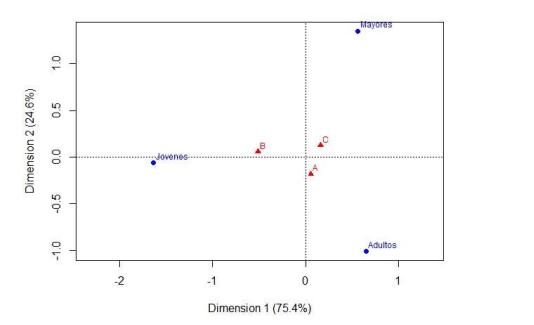
\includegraphics[width=\textwidth]{assets/grafico_asimetrico.png}
    \end{figure}
    
    \newpage

    \item \textbf{Mapas simétricos:} Son los más habituales. En esta ocasión tanto las filas como las columnas se representan en sus coordenadas principales (las obtenidas del análisis). No se pueden interpretar las distancias entre perfiles filas y columnas, ya que originalmente son espacios distintos e incluso podrían tener diferente dimensión.
    \item Se puede pasar del gráfico asimétrico al simétrico realizando una ``contracción'' igual a la raiz cuadrada del autovalor correspondiente a cada eje (no entendi nada xd).
    \begin{figure}[ht]
        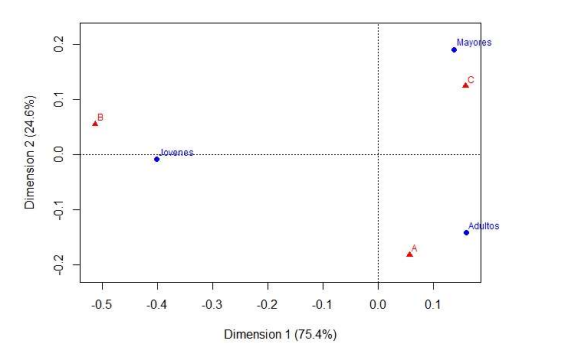
\includegraphics[width=\textwidth]{assets/grafico_simetrico.png}
    \end{figure}
    
    Vemos que a pesar de parecer ``cercanos'' Jovenes y el producto B, al no poder sacar conclusiones, sería injustificado decir que \textit{los jovenes prefieren el producto B}, y además, en este ejemplo, falso.
    \item \textbf{Biplots:} Solo se representa uno de los conjuntos en coordenadas principales. Los mapas asimétricos son un ejemplo de biplot, pero hay más tipos, como el biplot estandar.
    \begin{figure}[ht]
        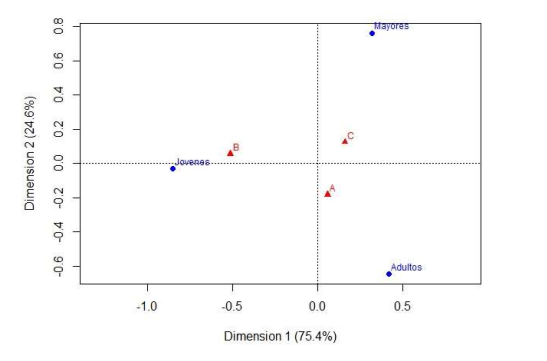
\includegraphics[width=\textwidth]{assets/grafico_biplot.png}
    \end{figure}
    \item No pueden interpretarse las distancias entre los puntos no representados en coordenadas principales, pero estos indican las direcciones de los ejes del biplot, y las coordenadas principales representadas sobre estos ejes si que son indicativas de la distancia entre esos puntos y la clase correspondiente a ese vértice.

    \newpage

    \item En la práctica aparecen casos típicos, los más comunes son los siguientes:
    \begin{itemize}
        \item Existencia de una asociación entre grupos de clases de las filas y grupos de clases de las columnas. Esto genera una representación en la que aparecen nubes de puntos separadas entre si donde están agrupadas las clases de fila y columna entre las que existe dicha asociación.
        \begin{figure}[ht]
            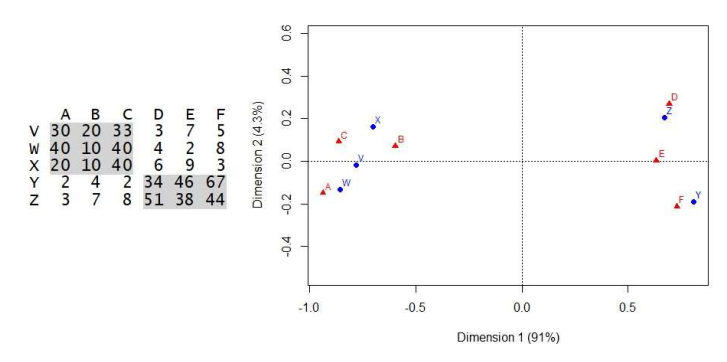
\includegraphics[width=\textwidth]{assets/asociacion_gruopos1.png}
        \end{figure}
        \begin{figure}[ht]
            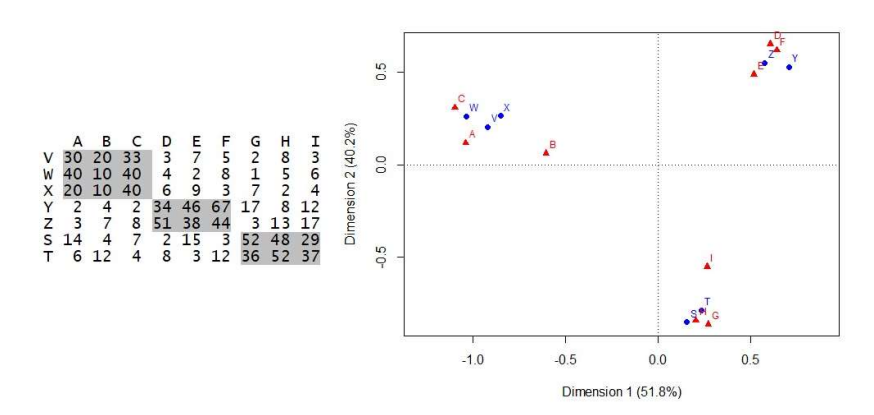
\includegraphics[width=\textwidth]{assets/asociacion_gruopos2.png}
        \end{figure}
        \newpage
        \vspace*{15mm}
        \item Existencia de una asociación fuerte entre dos variables categóricas que se analizan. De modo que los valores altos de la tabla de contingencia aparecen en la diagonal, y los puntos en los gráficos sigen el ``Efecto Guttman'' formando una nube con forma de parabola.
        \begin{figure}[ht]
            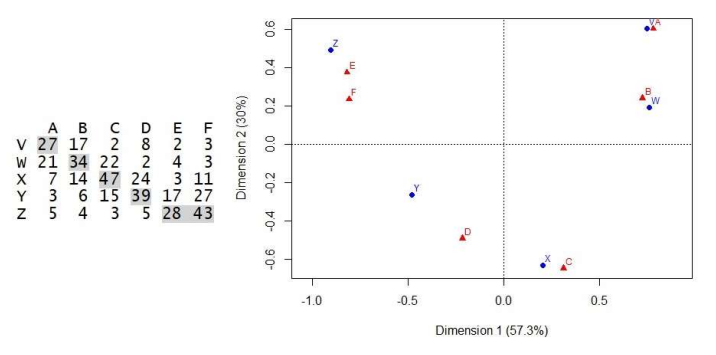
\includegraphics[width=\textwidth]{assets/asociacion_guttman.png}
        \end{figure}
        \newpage
        \item Existencia de una relación circular. Se relacionan en el mismo sentido valores altos y bajos.
        \begin{figure}[ht]
            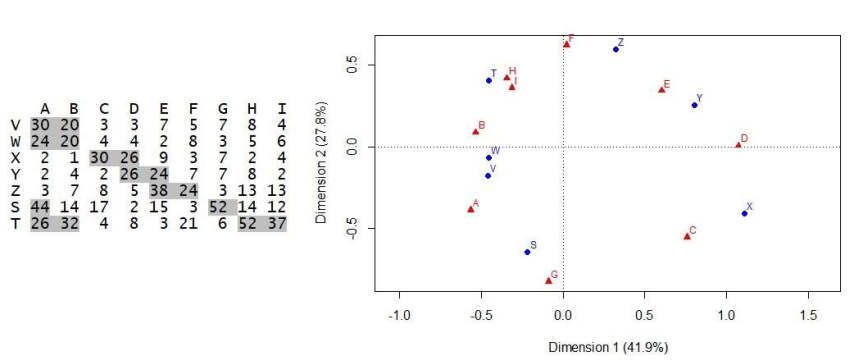
\includegraphics[width=\textwidth]{assets/asociacion_circular.png}
        \end{figure}
    \end{itemize}
    \item Se pueden añadir, igual que en ACP, elementos suplementarios (columnas o filas). Los elementos suplementarios corresponen a observaciones posteriores, en condiciones distintas, de naturaleza distinta\dots.
    \item Se proyectan en el análisis y se interpretan por proximidad a los elementos activos.
    \item No tienen contribuciones absolutas pero si relativas.
    \item Para hacer las proyecciones se utilizan las relaciones de transición o los factores.
    \item Proyecciones de elemntos suplementarios sobre el eje alpha:
    \[
        \text{Columna suplementaria:} \quad \hat{\varphi}^{+}_\alpha=\frac{1}{\sqrt{\lambda_\alpha}}\sum_{i=1}^r\left(\frac{n^{+}_i}{n^{+}_{+}}\right)\hat{\psi}_{\alpha i}=\sum_{i=1}^r\left(\frac{n^{+}_{i}}{n^{+}_{+}}\right)\psi_{\alpha i}
    \]
    \[
        \text{Fila suplementaria:} \qquad\quad \hat{\psi}^{+}_\alpha=\frac{1}{\sqrt{\lambda_\alpha}}\sum_{j=1}^c\left(\frac{n^{+}_j}{n^{+}_{+}}\right)\hat{\varphi}_{\alpha j}=\sum_{j=1}^c\left(\frac{n^{+}_{j}}{n^{+}_{+}}\right)\varphi_{\alpha j}
    \]
    \item Una de las aplicaciones del AC es asignar valores numéricos a las categorías de las variables implicadas.
    \item Sean $z_c(1),\dots,z_c(c)$ los valores numéricos a asignar a las $c$ categorías de una variable e $Y$ la variable que define las columnas de la tabla de contingencia.
    \item Esta asignación también determina la asignación de las $r$ categorías de $X$, variable que define las filas de la tabla de contingencia, ya que podemos asignar a la fila $i$ $\forall i=1,\dots,r$ el promedio con pesos de los valores $z_c(j)$ en esa fila:
    \[
        z_r(i)=\frac{\sum_{j=1}^c f_{ij}z_c(j)}{\sum_{j=1}^c f_{ij}}=\sum_{j=1}^c \frac{f_{ij}}{f_{i+}}z_c(j)
    \]
    \newpage
    \item $z_r=D^{-1}_rFz_c$
    \item $z_c=D^{-1}_cF'z_r$
    \item Juntando las anteriores ecuaciones queda
    \[
        z_r=D^{-1}_rFD^{-1}_cF'z_r
    \]
    \[
        z_c=D^{-1}_cF'D^{-1}_rFz_c
    \]
    Por lo que los vectores $z_r$ y $z_c$ son autovectores de las matrices $D^{-1}_rFD^{-1}_cF'$ y $D^{-1}_cF'D^{-1}_rF$ respectivamente.
    \item Estos autovectores ya están calculados, son $u_\alpha$ y $v_\alpha$ respectivamente.
    \item La asignación de puntuaciones es equivalente a la busqueda de la mejor proyección de los puntos.
    \item Una forma consistente de asignar dichas puntuaciones es tomar las proyecciones de dichas filas y columnas sobre el primer eje principal correspondiente.
    \item \textbf{Tablas de multiples entradas: } En ocasiones se tienen dos o más variables categóricas, e interesa tratar relaciones entre ellas, pero no entre todas. En estos casos se acomodan las variables en una única tabla de contingencia.
    
    \vspace*{2mm}

    \begin{tabular}{|c|c|c|c|c|c|}
        \hline
        Edad    &  MB  &  B  &  R  &  M  &  MM  \\
        \hline
        16-24   &  243 & 789 & 167 &  18 &    6 \\
        25-34   &  220 & 809 & 164 &  35 &    6 \\
        35-44   &  147 & 658 & 181 &  41 &    8 \\
        45-54   &   90 & 469 & 236 &  50 &   16 \\
        55-64   &   53 & 414 & 306 & 106 &   30 \\
        65-74   &   44 & 267 & 284 &  98 &   20 \\
        75+     &   20 & 136 & 157 &  66 &   17 \\
        \hline
    \end{tabular}
    \smallskip
    \begin{tabular}{|c|c|c|c|c|c|}
        \hline
        Sexo    &  MB  &   B  &  R  &  M  &  MM  \\
        \hline
        Hombre  &  448 & 1789 & 636 & 177 &   39 \\
        Mujer   &  369 & 1753 & 859 & 237 &   64 \\
        \hline
    \end{tabular}
    
    Representamos en una nueva tabla las variables cruzadas

    \begin{center}
        \begin{tabular}{|c|c|c|c|c|c|}
            \hline
            Sexo x Edad &  MB  &  B  &  R  &  M  &  MM  \\
            \hline
            h16-24      &  145 & 402 &  84 &   5 &   3 \\
            h25-34      &  112 & 414 &  74 &  13 &   2 \\
            h35-44      &   80 & 331 &  82 &  24 &   4 \\
            h45-54      &   54 & 231 & 102 &  22 &   6 \\
            h55-64      &   30 & 219 & 119 &  53 &  12 \\
            h65-74      &   18 & 125 & 110 &  35 &   4 \\
            h75+        &    9 &  67 &  65 &  25 &   8 \\
            m16-24      &   98 & 387 &  83 &  13 &   3 \\
            m25-34      &  108 & 395 &  90 &  22 &   4 \\
            m35-44      &   67 & 327 &  99 &  17 &   4 \\
            m45-54      &   36 & 237 & 134 &  28 &  10 \\
            m55-64      &   23 & 195 & 187 &  53 &  18 \\
            m65-74      &   26 & 142 & 174 &  63 &  16 \\
            m75+        &   11 &  69 &  92 &  41 &   9 \\
            \hline
        \end{tabular}
    \end{center}
    
    \item \textbf{Tablas concatenadas:} En los casos en los que tengamos muchas variables realizar el procedimiento anterior implicaria un exceso de categorías que haría imposible el análisis. En estos casos suelen usarse \textbf{tablas concatenadas}, donde las tablas de contingencia simplemente se apilan.
    \begin{figure}[h]
        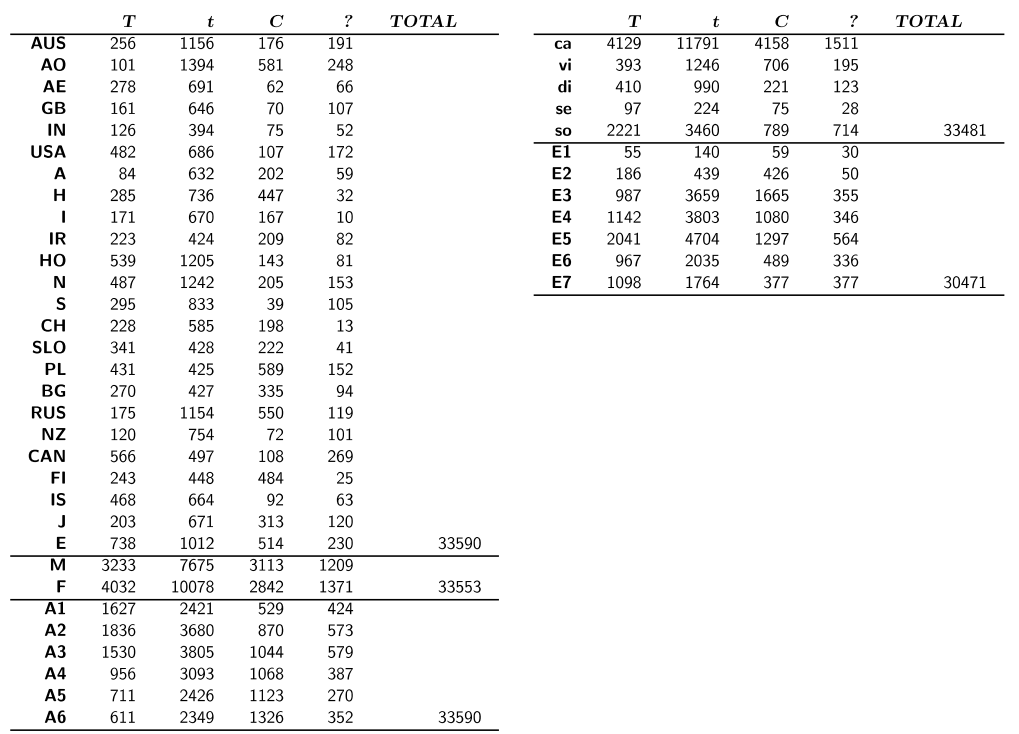
\includegraphics[width=\textwidth]{assets/tablas_apiladas.png}
    \end{figure}
    
    Podemos ver que, si quisiesemos representar el cruce de todas las variables tendríamos $24\cdot2\cdot6\cdot5\cdot7=10080$ categorías frente a las $24+2+6+5+7=44$ que estamos representando ahora.
\end{itemize}

\begin{wrapfigure}{l}{0.5\textwidth}
    \centering
    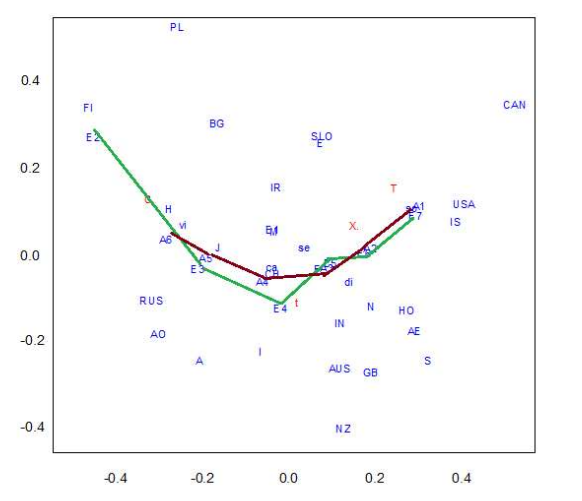
\includegraphics[width=0.5\textwidth]{assets/resultados_concatenadas.png}
\end{wrapfigure}

\noindent Con dos autovalores alcanzamos un 91.2\% de inercia explicada. La interpretación del primer eje que recoge el 63.4\% parece bastante clara. La del segundo es menos directa. Países en la parte alta tienen opiniones más polarizadas y los de abajo más frecuencia en las opiniones intermedias. 

\vspace*{5mm}

\noindent Se puede comprobar además que, si no hay datos ausentes, la inercia de la tabla concatenada es el promedio de las inercias de cada una de las tablas que se han agrupado.

\clearpage

\begin{itemize}
    \item Llamamos $T$ a la tabla completa y $T_1,\dots,T_s$ a las tablas que se agrupan.
    \item $\chi^2_T=\sum_{i=1}^s\chi^2_{T_i}$
    \item Por tanto la inercia total será
    \[
        \text{inercia}(T)=\frac{1}{s}\sum_{i=1}^s\text{inercia}(T_i)
    \]
    \item Tambien se pueden realizar concatenaciones por columnas
    \item \textbf{Análisis de correspondencias múltiples:} El caso en el que se tratan simultaneamente más de dos variables categóricas se denomina análisis de correspondencias múltiples (ACM).
    \item Se tienen $n$ individuos sobre $p$ variables categóricas.
    \item $j_q$ $\forall q=1,\dots,p$ es el número de categorías para la variable $q$.
    \item $J=\sum_{q=1}^p=j_q$.
    \item Los datos vienen representados en una matriz $R=(r_{iq})$ de dimensiones $n\times p$ denominada tabla de modalidades.
    \item El elemento $(i,q)$ contiene la categoría dada por el individuo $i$ en la variable $q$.
    \item Para analizar los datos se construye la matriz binaria (o tabla disyuntiva completa) $Z$ de dimensiones $n\times J$.
    \item $Z=[Z_1,\dots|Z_p]$ donde $Z_q=(z^q_{ij})$ $\forall q=1,\dots,p$ que es una matriz de dimensiones $n\times j_q$ en la que $z^q_{ij}=1$ si la respuesta del individuo $i$ para la variable $q$ ha sido la modalidad $j$ de dicha variable, o 0 en caso contrario.
    \item La \textbf{primera opción} para efectuar un ACM es hacer un AC sobre la matriz binaria $Z$.
    \item $\chi^2_{Z_q}=\sum_{i=1}^{j_q}n(j_q-1)$
    \item $\text{inercia}(Z)=\frac{1}{p}\sum_{q=1}^p\text{inercia}(Z_q)$
    \item Por tanto
    \[
        \text{inercia}(Z)=\frac{1}{p}\sum_{q=1}^p\frac{n(j_q-1)}{n}=\frac{J-p}{p}
    \]
    \newpage
    \item La \textbf{segunda opción} para efectuar un ACM es utilizar la matriz de Burt, que se define como $B=Z'Z$ y tendrá dimensiones $J\times J$ que tiene la forma
    \[
        \begin{bmatrix}
            D_1     & F_{12}  & \cdots & F_{1p} \\
            F'_{12} & D_2     & \cdots & F_{2p} \\
            \vdots  & \vdots  & \ddots & \vdots \\
            F'_{1p} & F'_{2p} & \cdots & D_p
        \end{bmatrix}
    \]

    donde $D_q$ es una matriz diagonal que contiene la distribución marginal de la variable $q$ y $F_{qr}$ es la tabla de contingencia de las variables $q$ y $r$.
    \item Los autovalores obtenidos del análisis de $B$ serán el cuadrado de los autovalores obtenidos con la matriz binaria $Z$
    \item La inercia total es igual al promedio de las inercias de las $p\times p$ submatrices que la componen, y además, la inercia de las matrices diagonales $D_q$ es igual a $j_q-1$.
    \item Las coordenadas factoriales son un reescalado de las obtenidas a partir de la tabla binaria $\varphi_{B,\alpha}(j)=\sqrt{\lambda_{Z,\alpha}}\varphi_{Z,\alpha}(j)$
    \item Los porcentajes de inercia explicados por el análisis de Burt siempre serán superiores a los obtenidos con el otro método.
    \begin{table}[h!]
        \centering
        \resizebox{\textwidth}{!}{
    
        \begin{tabular}[width=\textwidth]{c|cccc|cccc|cccc|cccc|}       
                 & Q1.1 & Q1.2 & Q1.3 & Q1.4 & Q2.1 & Q2.2 & Q2.3 & Q2.4 & Q3.1 & Q3.2 & Q3.3 & Q3.4 & Q4.1 & Q4.2 & Q4.3 & Q4.4 \\
            \hline
            Q1:1 & 2501 & 0    & 0    & 0    & 172  & 1107 & 1131 & 91   & 355  & 1710 & 345  & 91   & 1766 & 538  & 40   & 157  \\
            Q1:2 & 0    & 476  & 0    & 0    & 7    & 129  & 335  & 5    & 16   & 261  & 181  & 18   & 128  & 293  & 17   & 38   \\
            Q1:3 & 0    & 0    & 79   & 0    & 1    & 6    & 72   & 0    & 1    & 17   & 61   & 0    & 14   & 21   & 38   & 6    \\
            Q1:4 & 0    & 0    & 0    & 362  & 1    & 57   & 108  & 196  & 7    & 96   & 205  & 4    & 45   & 45   & 2    & 264  \\
            \hline
            Q2:1 & 172  & 7    & 1    & 1    & 181  & 0    & 0    & 0    & 2    & 165  & 15   & 0    & 0    & 0    & 0    & 1    \\
            Q2:2 & 1107 & 129  & 6    & 57   & 0    & 127  & 0    & 0    & 219  & 997  & 61   & 22   & 972  & 239  & 13   & 75   \\
            Q2:3 & 1131 & 335  & 72   & 108  & 0    & 0    & 1646 & 0    & 24   & 989  & 573  & 60   & 760  & 616  & 84   & 186  \\
            Q2:4 & 91   & 5    & 0    & 196  & 0    & 0    & 0    & 292  & 59   & 4    & 229  & 62   & 60   & 30   & 0    & 234  \\
            \hline
            Q3:1 & 355  & 16   & 1    & 127  & 219  & 24   & 9    & 379  & 642  & 0    & 0    & 0    & 1    & 1    & 1    & 4    \\
            Q3:2 & 1710 & 261  & 17   & 96   & 48   & 997  & 989  & 50   & 0    & 2084 & 0    & 0    & 1348 & 567  & 23   & 146  \\
            Q3:3 & 345  & 181  & 61   & 55   & 4    & 61   & 573  & 4    & 0    & 0    & 313  & 0    & 202  & 286  & 73   & 81   \\
            Q3:4 & 91   & 18   & 0    & 204  & 2    & 22   & 60   & 0    & 0    & 0    & 0    & 49   & 30   & 0    & 0    & 234  \\
            \hline
            Q4:1 & 1766 & 128  & 14   & 51   & 165  & 972  & 760  & 62   & 360  & 1348 & 202  & 49   & 1959 & 0    & 0    & 0    \\
            Q4:2 & 538  & 293  & 21   & 45   & 15   & 239  & 616  & 27   & 14   & 567  & 286  & 30   & 0    & 897  & 0    & 0    \\
            Q4:3 & 40   & 17   & 38   & 2    & 0    & 1    & 0    & 0    & 23   & 0    & 0    & 0    & 0    & 0    & 97   & 0    \\
            Q4:4 & 157  & 38   & 6    & 264  & 1    & 75   & 186  & 203  & 4    & 146  & 81   & 234  & 0    & 0    & 0    & 465  \\
            \hline
        \end{tabular}
        }
        \caption{Ejemplo de tabla de Burt}
    \end{table}
    \item Corrección de los autovalores:
    \[
        \lambda^{\text{adj}}_\alpha=\left(\frac{p}{p-1}\right)^2\left(\sqrt{\lambda^B_\alpha}-\frac{1}{p}\right)^2
    \]
    \item En la Corrección de Benzerí se calculan los porcentajes de inercia correspondiente a cada eje dividiendo por la suma de los autovalores corregidos.
    \item En la Corrección de Greenacre para calcular los porcentajes se divide por la inercia total descontando la de las tablas diagonales. 
    
    Se puede calcular como $\frac{p}{p-1}\left(\text{inercia}(B)-\frac{J-p}{p^2}\right)$.
    \begin{figure}[ht]
        \centering
        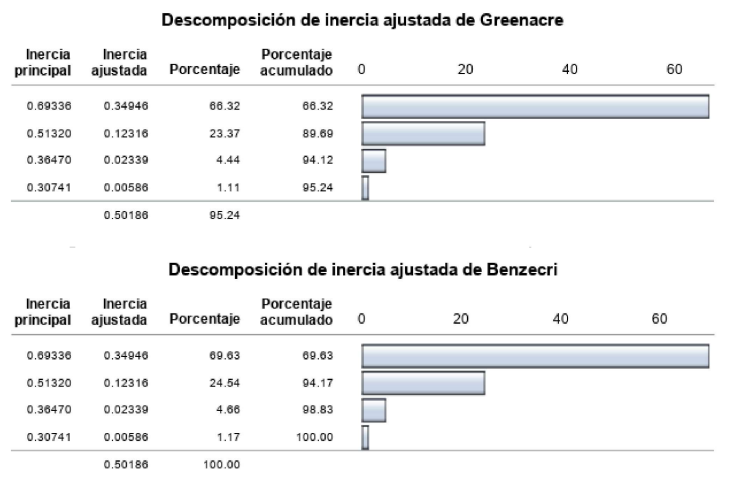
\includegraphics[width=\textwidth]{assets/correcciones_inercia.png}
    \end{figure}
\end{itemize}


\section{Clasificaci\'on Supervisada: An\'alisis Discriminante}

\begin{itemize}
    \item Tablas de datos con $n$ individuos, $p$ variables y una variable categórica $G$ con $q$ niveles.
    
    \begin{center}
        \begin{tabular}{|cccc|c|}
            \hline
               $X_1$ &    $X_2$ & $\cdots$ &    $X_p$ &      $G$ \\
            \hline
            $x_{11}$ & $x_{12}$ & $\cdots$ & $x_{1p}$ &    $g_1$ \\
            $x_{21}$ & $x_{22}$ & $\cdots$ & $x_{2p}$ &    $g_2$ \\
            $\vdots$ & $\vdots$ & $\ddots$ & $\vdots$ & $\vdots$ \\
            $x_{n1}$ & $x_{n2}$ & $\cdots$ & $x_{np}$ &    $g_n$ \\
            \hline
        \end{tabular}
    \end{center}

    \item El objetivo es determinar para un nuevo paciente $x_{(n+1)}$ con $X_1=x_{(n+1)1},\dots,X_p=x_{(n+1)p}$ su clasificación en $G$.
    \item \textbf{Muestra patrón:} Se llama muestra patrón (o \textit{train-data}) al conjunto de observaciones pareadas con su grupo. $\mathcal{Z}=\{x_i,g_i\}_{i=1}^n$
    \item \textbf{Regla de Bayes:} Asignaremos $x$ al grupo $K$ si
    \[
        \pi_Kf_K(x)=\max_{k=1,\dots,q}\pi_kf_k(x)
    \]
    \item Se utiliza la información disponible en $\mathcal{Z}$ para obtener $\hat{\pi}_k$ y $\hat{f}_k(x)$.
    \item \textbf{Normal multivariante:} $X=(X_1,\dots,X_p)'$ sigue una distribución normal $p$-variante $X\sim N_p(\mu,\Sigma)$ si admite densidad
    \[
        f(x;\mu,\Sigma)=\frac{1}{(2\pi)^{p/2}|\Sigma|^{1/2}}\text{exp}\left\{-\frac{1}{2}(x-\mu)'\Sigma^{-1}(x-\mu)\right\} \quad \forall x \in \mathbb{R}^p
    \]
    \item Elipsoides de equidensidad: $\{x:(x-\mu)'\Sigma^{-1}(x-mu)=\text{cte.}\}$
    \item \textbf{Distancia de Mahalanobis:} Mide la distancia de $x$ al centro de la distribución $\mu$ teniendo en cuenta la ``estructura de dispersión'' dada por $\Sigma$
    \[
        d(x;\mu,\Sigma)=\sqrt{(x-\mu)'\Sigma^{-1}(x-\mu)}
    \]
    \item \textbf{Regla discriminante lineal para $q=2$:} Suponiendo poblaciones normales y $\Sigma_1=\Sigma_2=\Sigma$ asigmanos $x$ al grupo 2 si
    \[
        \pi_2f_2(x)>\pi_1f_1(x)
    \]
    \item \textbf{Costes asimétricos:} Si $c(i|j)$ es el coste de clasificar una observación del grupo $j$ en el grupo $i$ la Regla de Bayes cambia a
    \[
        \text{asignar al grupo 2 si} \quad \frac{\pi_2f_2(x)}{c(2|1)}>\frac{\pi_1f_1(x)}{c(1|2)}
    \]
    \item $\{1,2,3,\dots,n\}=I_1\cup\dots\cup I_q$ con $\#I_k=n_k$ y $n_1+\cdots+n_q=n$.
    \newpage
    \item \textbf{Reglas muestrales:} Los parámetros $\mu_j$ y $\Sigma$ se estiman
    \begin{itemize}
        \item $\hat{\mu}_k=\frac{1}{n_k}\sum_{i\in I_k}x_i$
        \item $\hat{\Sigma}_k=\frac{1}{n_k-1}\sum_{i\in I_k}(x_i-\hat{\mu}_k)(x_i-\hat{\mu}_k)'$
        \item $\hat{\Sigma}=\frac{1}{n-q}\sum_{k=1}^q(n_k-1)\hat{\Sigma}_k$
        \item $\hat{\pi}_k=\frac{n_k}{n}$
    \end{itemize}
    \item \textbf{Coordenadas Discriminantes de Fisher:} Mejores proyecciones en el sentido de que los grupos estén separados y sean homogeneos en el espacio proyectado.
    \item Notación:
    \begin{itemize}
        \item $\overline{x}^j=\frac{1}{n}\sum_{i=1}^nx_{ij}$ es la media de la variable $j$.
        \item $\overline{x}^j_k=\frac{1}{n_k}\sum_{i\in I_k}x_ij$ es la media de la variabe $j$ en el grupo $k$.
    \end{itemize}
    \item $T=W+B$ donde $T$ es el ``Total'' \textit{(Total)}, $W$ es ``dentro'' \textit{(Within)} y $B$ es ``entre'' \textit{(Between)}.
    \item $T_{jj'}=\frac{1}{n}\sum_{i=1}^n(x_{ij}-\overline{x}^j)(x_{ij'}-\overline{x}^{j'})$ que se descompone en
    \[
        \underbrace{\frac{1}{n}\sum_{k=1}^q\sum_{i\in I_k}(x_{ij}-\overline{x}^{j_k})(x_{ij'}-\overline{x}^{j'_k})}_W + \underbrace{\sum_{k=1}^q\frac{n_k}{n}(\overline{x}^j_k-\overline{x}^j)(\overline{x}^{j'}_k-\overline{x}^{j'})}_B
    \]
    \item En $u'Tu=u'Wu+u'Bu$ se busca maximizar $u'Bu$ (\textit{dispersión entre grupos}) y minimizar $u'Wu$ (\textit{dispersión dentro grupos}).
    \item La \textbf{mejor proyección} viene dada por $u_1$ autovector de $W^{-1B}$ asociado al autovalor mayor. El resto de autovectores $u_2,\dots,u_d$ recogen la siguiente mejor proyección en función de sus autovalores asociados.
    \item Sea $t(z)=(t_1(z),\dots,t_d(z))'$ para $z=(z_1,\dots,z_p)'$ y con $t_j(z)=u'_jz$ la \textbf{función discriminante}.
    \item Sea $\overline{x}_k=(\overline{x}^1_k,\dots,\overline{x}^p_k)$ el centroide del grupo $k$. Se \textbf{asigna una nueva observación $z$} al grupo $K$ cuando
    \[
        \|t(z-\overline{x}_K)-t(\overline{x}_K)\|=\inf_{k=1,\dots,q}\|t(z-\overline{x}_k)-t(\overline{x}_k)\|
    \]
    IMPORTANTE CENTRAR LA OBSERVACIÓN.
    \item $d\leq \min\{q-1,p\}$
    \item El enfoque de fisher para $q=2$, misma varianza y mismas probabilidades a priori coincide con el discriminante lineal.
    \newpage
    \item \textbf{Discriminación Cuadrática:} Se permite $\Sigma_1\neq\Sigma_2$ en los grupos.
    \item Se puede aproximar con LDA con variables $x^2_1,\dots,x^2_p,x_1x_2,\dots,x_1x_p,\dots$.
    \item El número de parámetros incrementa drásticamente con $p$, lo que puede llevar a sobreajustes.
    \item \textbf{Naive Bayes:} Se asume que las variables predictoras son independientes.
    \item Permite estimar $f_kj$ mediante técnicas de suavizado, entre otras (no obliga a que $f \sim N(\mu, \sigma^2)$).
    \item \textbf{Tabla de clasificación:} Se cruzan las clasificaciones reales con las predichas. Los valores en la diagonal están ``bien'' clasificados, los de fuera no.
    
    \begin{center}
        \begin{tabular}{l|lcccl|}
            \cline{2-6}
                                                        & \multicolumn{5}{l|}{Predicción}                                                                                     \\ \hline
            \multicolumn{1}{|l|}{\multirow{5}{*}{Real}} & \multicolumn{1}{c|}{}      & \multicolumn{1}{c|}{$k_1$}      & \multicolumn{1}{c|}{$k_2$}      & \multicolumn{1}{c|}{$\cdots$} & $k_q$      \\ \cline{2-6} 
            \multicolumn{1}{|l|}{}                      & \multicolumn{1}{c|}{$k_1$} & \multicolumn{1}{c|}{\ding{51}} & \multicolumn{1}{c|}{\ding{55}}           & \multicolumn{1}{c|}{$\cdots$} & \ding{55}           \\ \cline{2-6} 
            \multicolumn{1}{|l|}{}                      & \multicolumn{1}{c|}{$k_2$} & \multicolumn{1}{c|}{\ding{55}}          & \multicolumn{1}{c|}{\ding{51}} & \multicolumn{1}{c|}{$\cdots$} &  \ding{55}          \\ \cline{2-6} 
            \multicolumn{1}{|l|}{}                      & \multicolumn{1}{l|}{$\vdots$}   & \multicolumn{1}{l|}{$\vdots$}        & \multicolumn{1}{l|}{$\vdots$}        & \multicolumn{1}{l|}{$\ddots$} & $\vdots$        \\ \cline{2-6} 
            \multicolumn{1}{|l|}{}                      & \multicolumn{1}{l|}{$k_q$} & \multicolumn{1}{l|}{\ding{55}}          & \multicolumn{1}{l|}{\ding{55}}           & \multicolumn{1}{l|}{$\cdots$} & \ding{51} \\ \hline
        \end{tabular}
    \end{center}

    \item Tipos de error:
    \[
        \text{Sensibilidad:} \quad \frac{VP}{VP+FN}=\frac{VP}{P}
    \]
    \[
        \text{Especificidad:} \quad \frac{VN}{VN+FP}=\frac{VN}{N}
    \]
    \item \textbf{Error Aparente:} Es la proporción de mal clasificados al probar la regla en $\mathcal{Z}$.
    \[
        \overline{\text{err}}=\frac{1}{n}\sum_{i=1}^n\{\hat{G}(x_i)\neq g_i\}
    \]
    \item Estimación optimista de la verdadera tasa de error.
    \item Premia modelos sobreajustados.
    \item \textbf{Error de generalización:} Error esperado para una nueva observación aleatoria
    \[
        Err_{\mathcal{Z}}=E_{(X,G)[L(\hat{G}(X),G)|\mathbfcal{Z}=\mathcal{Z}]}
    \]
    \item \textbf{Error esperado de generalización:}
    \[
        Err=E[Err_{\mathcal{Z}}]
    \]
    \newpage
    \item Sobreajuste e subajuste:
    \begin{itemize}
        \item ``Sobreajuste'': Modelos excesivamente complejos (demasiadas variables o excesiva flexibilidad)
        \item ``Subajuste'': Modelos más simples de lo necesario (pocas variables informativas o poca flexibilidad)
    \end{itemize}
    \begin{figure}[ht]
        \centering
        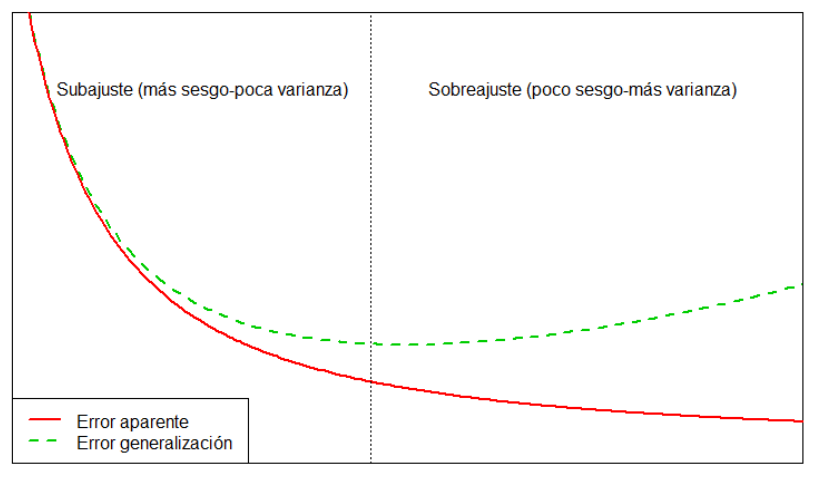
\includegraphics[width=\textwidth]{assets/overfitting_underfitting.png}
    \end{figure}
    \item \textbf{Validación cruzada:} Se pretende estimar el error esperado de generalización para comparar modelos.
    Se realiza una partición de la muestra patrón $\mathcal{Z}=\begin{pmatrix}\mathcal{Z}_1 \\ \mathcal{Z}_2\end{pmatrix}$ y se usarán solo las observaciones en $\mathcal{Z}_1$ para ajustar la regla y se comprobará con $\mathcal{Z}_2$. A continuación se exponen algunos métodos de \textbf{validación cruzada}
    \begin{itemize}
        \item \textbf{$K$-fold:} $K$ bloques de la muestra patrón. Se usan $K-1$ bloques para ajustar la regla y el otro para validarla. Se promedian los errores.
        \item \textbf{Leave-one-out:} Una observación no se usa para entrenar, se realiza lo mismo para todas las observaciones y se promedia el error.
        \item \textbf{Muestra aleatoria:} Se toma una muestra aleatoria como partición de la muestra patrón, se ajusta con ella y se usa el resto de observaciones para estimar el error (``.632Bootstrap'', ``out-of-bag''\dots).
    \end{itemize}
    \item \textbf{$m$-vecinos más proximos:} Sean $N_m(x)$ las $m$ observaciones más próximas a $x$. Se seguirá un método de votación en el cual se asigna a $K$ si
    \[
        \#\{x_i\in N_m(x)\enspace \text{con} \enspace g_i=K\}=\max_{1\leq k\leq q}\#\{x_i\in N_m(x)\enspace \text{con} \enspace g_i=k\}
    \]
    \newpage
    Problemas de sobreajuste cuando $m$ es muy pequeño o de subajuste cuando $m$ es demasiado grande.
    \begin{figure}[h]
        \centering
        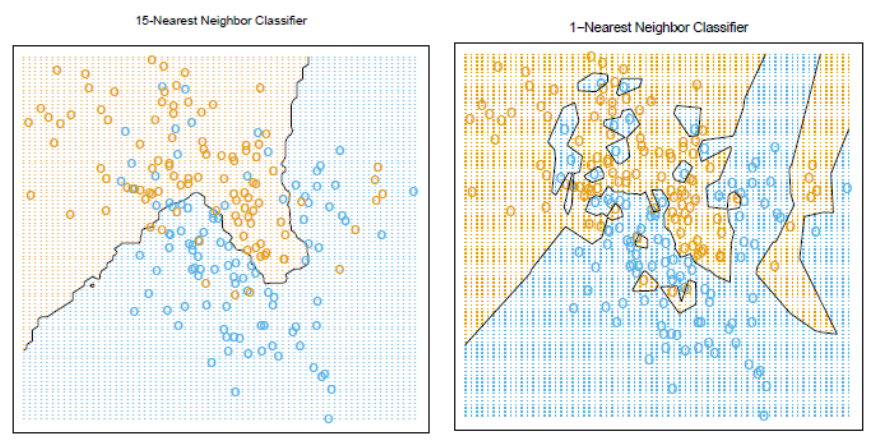
\includegraphics[width=\textwidth]{assets/k_neighbours.png}
    \end{figure}
    \item Árboles de clasificación: Son la base de métodos muy efectivos (Random Forest).
    \begin{figure}[h]
        \centering
        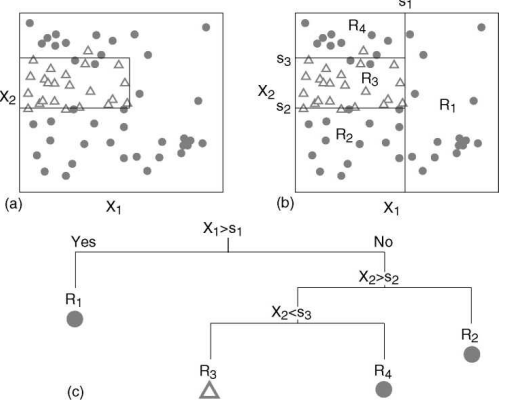
\includegraphics[width=0.8\textwidth]{assets/cart_classification.png}
    \end{figure}
    \newpage
    \item Suport Vector Machines (SVM): A partir de dos clases separables linealmente se busca el hiperplano que separa las clases con el mayor ``margen'' ($m$) posible.
    \begin{figure}[h]
        \centering
        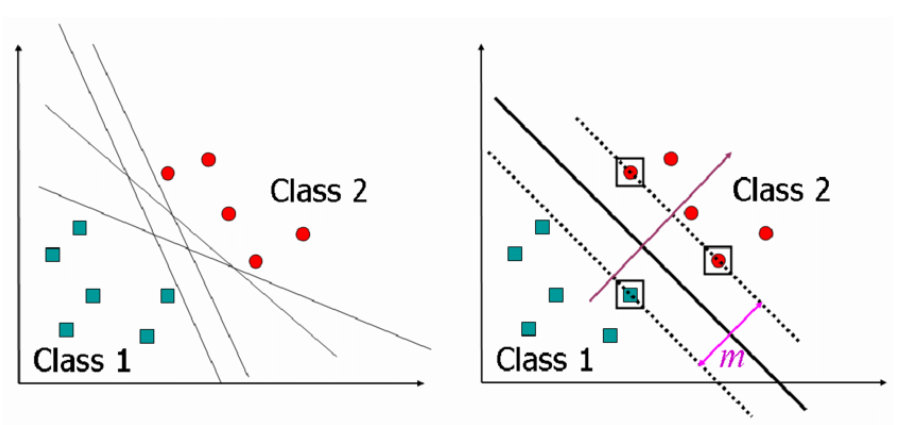
\includegraphics[width=\textwidth]{assets/svm_classification.png}
    \end{figure}
    
    En caso de que no sean separables se transforman los datos a un espacio de dimensión mayor donde si lo sean.
 \end{itemize}


\section{Clasificación no Supervisada: Análisis Cluster}

\begin{itemize}
    \item Agrupar $n$ individuos en grupos (clusters), tratando de que sean homogeneos en el grupo y con grupos heterogeneos entre si.
    \item Desconocemos la cantidad de grupos que se busca, ni existe una asignación previa en el conjunto de entrenamiento.
    \item \textbf{Métodos Jerárquicos:} Se define una expresión de disimilaridad y se asigna en grupos en función de la distancia, es decir, se ``ordenan'' en función de una/s regla/s (jerarquía).
    \item \textbf{Índice de disimilaridad} $d(x_i,x_{i'})$ mide diferencias entre individuos
    \begin{itemize}
        \item Euclidea: $d_E(x_i,x_{i'})=\|x_i-x_{i'}\|=\sqrt{(x_{i1}-x_{i'1})^2+\cdots+(x_{ip}-x_{i'p})^2}$.
        \item Manhatan o City Block: $d_M(x_i,x_{i'})=|x_{i1}-x_{i'1}|+\cdots|x_{ip}-x_{i'p}|$.
        \item Máximo o Chebyshev: $d_{Ch}(x_i,x_{i'})=\max\{|x_{i1}-x_{i'1}|,\dots,|x_{ip}-x_{i'p}|\}$.
        \item Camberra: Cuando las variables son positivas. $d_C(x_i,x_{i'})=\sum_{j=1}^p\frac{|x_{ij}-x_{i'j}|}{|x_{ij}|+|x_{i'j}|}$.
        \item 1-coseno: Siendo $\alpha$ el ángulo entre los vectores. $d_{\text{1-cos}}(x_i,x_{i'})=1-\cos(\alpha)$.
        
        Si trabajamos con datos ``normalizados'' al centrar por filas ($\tilde{x}_{ij}=x_{ij}-\overline{x}_i)$. $d_{\text{1-cos}}(\tilde{x}_i,\tilde{x}_{i'})=1-\text{Corr}(\tilde{x}_i,\tilde{x}_{i'})$.
        \item Single-matching, Jaccard, Tanimoto, Seath-Sokal: Para variables con niveles binarios.
        \item Distancias para variables categóricas, cadenas (Hamming y Levenshtein), variables mixtas (Gower)\dots
    \end{itemize}
    \item \textbf{Índice de agregación} $\partial(A,B)$ mide diferencias entre grupos
    \begin{itemize}
        \item Single Linkage: $\partial(A,B)=\min_{x\in A,y\in B}d(x,y)$. Afectado por problemas de ``cadena''
        \begin{figure}[h]
            \centering
            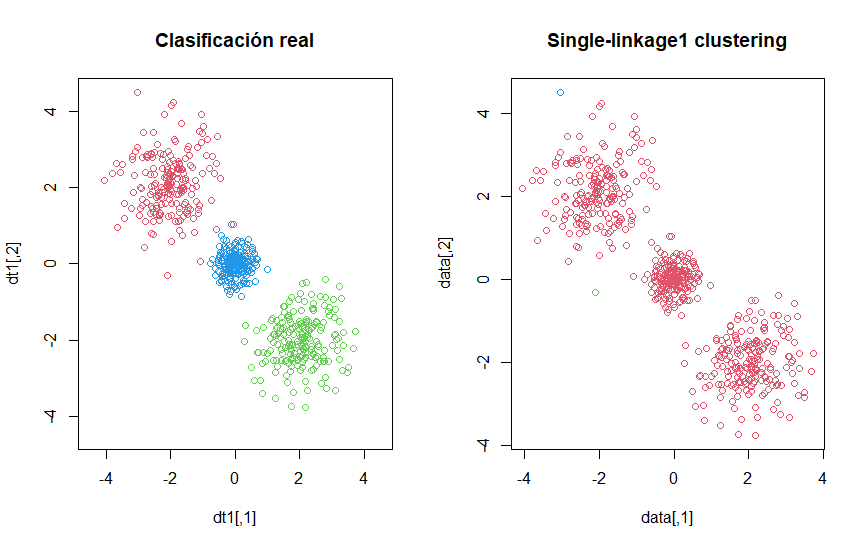
\includegraphics[width=0.8\textwidth]{assets/chain_effect.png}
        \end{figure}
        \newpage
        \item Complete linkage: $\partial(A,B)=\max_{x\in A,y\in B}d(x,y)$.
        \item Método de Ward: El individuo $x$ tiene peso $p(x)$. Si $n_C=\sum_{x\in C}p(x)$ y $g_C=\frac{1}{n_C}\sum_{x\in C}xp(x)$ entonces
        \[
            \partial(A,B)=\frac{n_A n_B}{n_A+n_B}d(g_A, g_B)^2
        \]
    \end{itemize}
    \item \textbf{Dendrograma:} Se unen $A$ y $B$ por etapas donde en cada etapa, $\partial(A,B)$ sea la más pequeña. Se repite el proceso hasta que no queden observaciones. Para crear los grupos se ``corta'' el árbol.
    \begin{figure}[h]
        \centering
        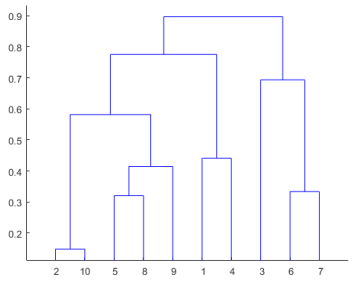
\includegraphics[width=0.5\textwidth]{assets/dendograma.png}
    \end{figure}
    \item \textbf{Métodos no Jerárquicos:} Se fija el número de grupos a buscar y se optimiza algún criterio, como por ejemplo la media de los grupos.
    \item \textbf{Método de $k$-medias:} Se buscan $k$ centros óptimos $m_1^*,\dots,m_k^*$ en $\mathbb{R}^p$.
    \item Algoritmo: Se seleccionan $k$ centros al azar $c_1^0,\dots,c_k^0$ y se crean particiones $I_1^0,\dots,I_k^0$ por cercanía. Despues se calcula la media de cada partición y se asignan como nuevos centros $c_1^1,\dots,c_k^1$. Se repite el proceso hasta estabilizarse ($I_j^{k-1}=I_j^k$).
    \begin{figure}[h]
        \centering
        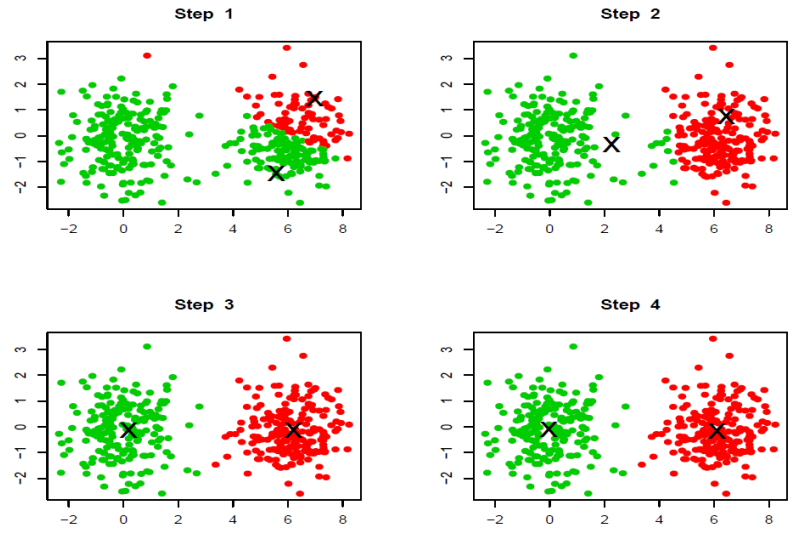
\includegraphics[width=0.8\textwidth]{assets/k_means.png}
    \end{figure}
    \newpage
    \item Las $k$-medias tienen preferencia por clusters esféricos y con dispersiones parecidas.
    \item \textbf{Métodos basados en modelos:} Métodos más flexibles, como la maximización de la verosimilitud de ``clasificación'' o la maximización de la verosimilitud tipo ``mixtura''.
    \item Las $k$-medias son un tipo especial de la maximización de la verosimilitud de ``clasificación''.
    \item Lo del final no se si ponerlo xd.
    \item Mapa de calor: Matriz de distancias. Representa en cada elemento $ij$ la distancia entre el individuo $i$ y el $j$ (lo pongo al final por que se me olvidó antes y asi relleno la página ole).
    \begin{figure}[h]
        \centering
        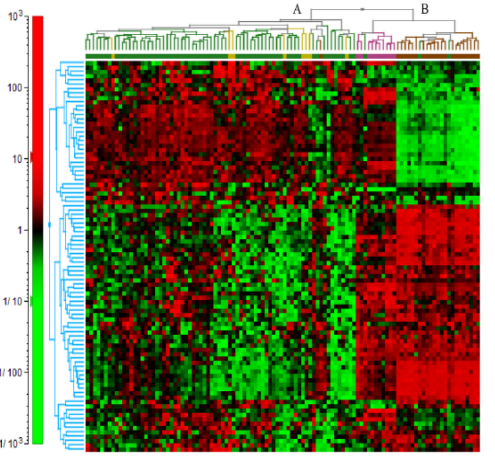
\includegraphics[width=\textwidth]{assets/mapa_calor.png}
    \end{figure}
\end{itemize}

% ------------------------------------------------------------------------------

\newpage

% ------------------------------------------------------------------------------
% Reference and Cited Works
% ------------------------------------------------------------------------------

\begin{thebibliography}{9}
    \bibitem{diapo1}
    Miguel Alejandro Fernández, \\ \textit{Diapositivas Análisis por Componentes Principales}. \\ Universidad de Valladolid, 2024.
    \bibitem{diapo2}
    Miguel Alejandro Fernández, \\ \textit{Diapositivas Análisis de Correspondencias}. \\ Universidad de Valladolid, 2024.
    \bibitem{diapo3}
    Luis Ángel García, \\ \textit{Diapositivas Clasificación Supervisada, Análisis Discriminante}. \\ Universidad de Valladolid, 2024.
    \bibitem{diapo4}
    Luis Ángel García, \\ \textit{Diapositivas Clasificación no Supervisada, Análisis Cluster}. \\ Universidad de Valladolid, 2024.
\end{thebibliography}

% ------------------------------------------------------------------------------

\end{document}
